\documentclass{standalone}

\usepackage{amssymb}
\usepackage{amsthm}
\usepackage{amsmath}


\usepackage{tikz}
\usetikzlibrary{shapes,backgrounds,calc,patterns}


\begin{document}
	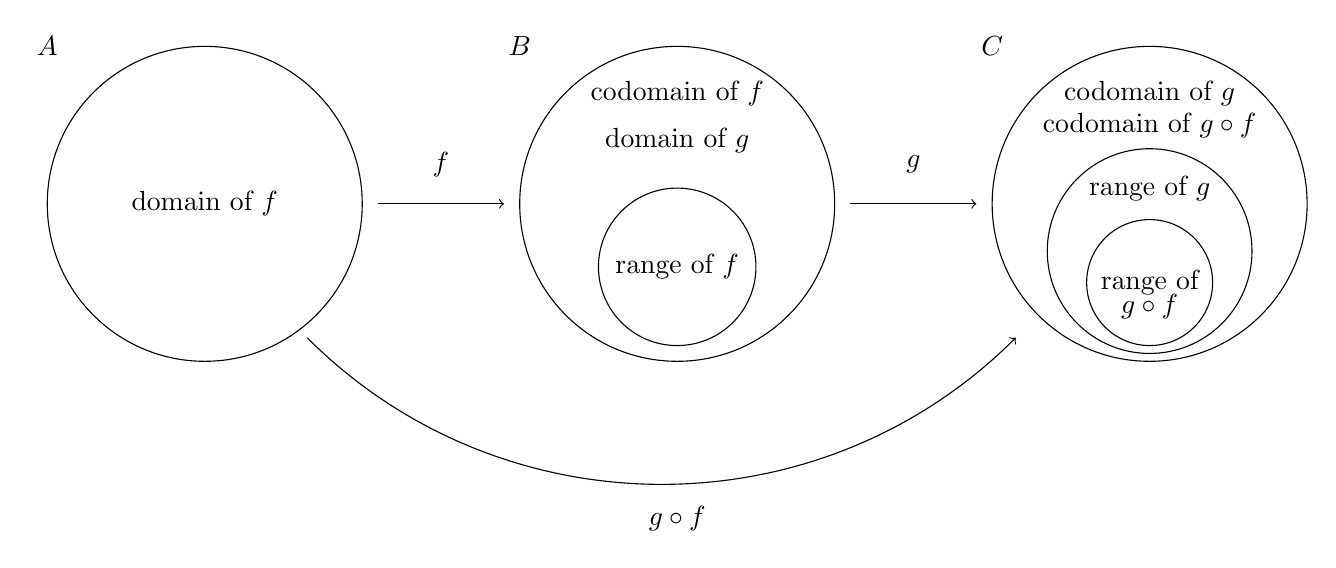
\begin{tikzpicture}
		\draw (-3,0) circle (2);
		\node at (-3,0) {domain of \(f\)};
		\node at (-5,2) {\(A\)};
		
		\draw (3,0) circle (2);
		\node at (3,1.4) {codomain of \(f\)};
		\node at (3,.8) {domain of \(g\)};
		\node at (1,2) {\(B\)};	
		
		\draw (3,-.8) circle (1);
		\node at (3,-.8) {range of \(f\)};

		
		\draw[->] (-.8,0) -- (.8,0);
		\node at (0,.5) {\(f\)};
		
		\draw (9,0) circle (2);
		\node at (9,1.4) {codomain of \(g\)};
		\node at (9,1) {codomain of \(g\circ f\)};
		\node at (7,2) {\(C\)};	

		\draw (9,-.6) circle (1.3);
		\node at (9,.2) {range of \(g\)};


		\draw (9,-1) circle (.8);
		\node at (9,-1) {range of};
		\node at (9,-1.3) {\(g\circ f\)};	
		
		\draw[->] (5.2,0) -- (6.8,0);
		\node at (6,.5) {\(g\)};
		
		\draw[->] (-1.7,-1.7) to[out=-45,in=225] (7.3,-1.7);
		\node at (3,-4) {\(g\circ f\)};		
	\end{tikzpicture}
	
	
	
\end{document}